% TikZ code representing a circuit computing the XOR function on two bits x_1 and x_2.
% Based on Figure 6.1 (page 107) of "Computational Complexity: A Modern Approach" (Arora & Barak).

\usetikzlibrary{arrows.meta}

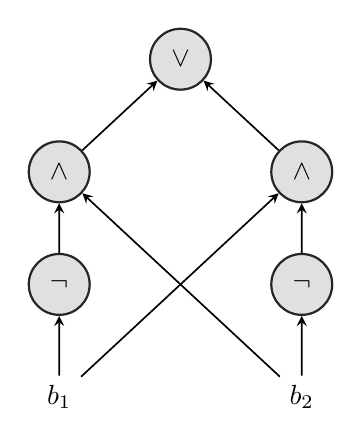
\begin{tikzpicture}[
    scale=1.1,
    gate/.style={circle, draw=black!85, fill=black!12, thick, minimum size=22pt, inner sep=0pt},
    arrow/.style={->, >=stealth, semithick}
]

    % Input nodes
    \node (x1) at (-1.4, 0) {$b_1$};
    \node (x2) at (1.4, 0) {$b_2$};

    % NOT gates
    \node[gate] (not1) at (-1.4, 1.3) {$\neg$};
    \node[gate] (not2) at (1.4, 1.3) {$\neg$};

    % AND gates
    \node[gate] (and1) at (-1.4, 2.6) {$\land$};
    \node[gate] (and2) at (1.4, 2.6) {$\land$};

    % OR gate (output)
    \node[gate] (or) at (0, 3.9) {$\lor$};

    % Edges from inputs to NOT gates
    \draw[arrow] (x1) -- (not1);
    \draw[arrow] (x2) -- (not2);

    % Edges to left AND gate
    \draw[arrow] (not1) -- (and1);
    \draw[arrow] (x2) -- (and1);

    % Edges to right AND gate
    \draw[arrow] (x1) -- (and2);
    \draw[arrow] (not2) -- (and2);

    % Edges to top OR gate
    \draw[arrow] (and1) -- (or);
    \draw[arrow] (and2) -- (or);

\end{tikzpicture}
